

\tikzset{every picture/.style={line width=0.75pt}} %set default line width to 0.75pt        

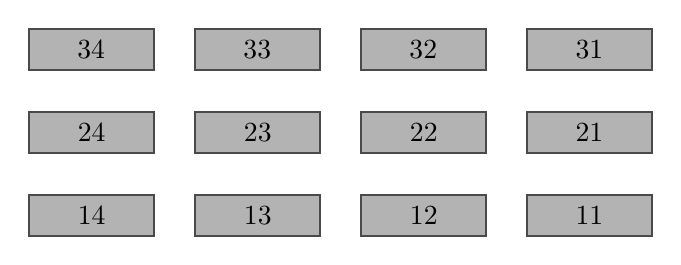
\begin{tikzpicture}[x=0.75pt,y=0.75pt,yscale=-1,xscale=1]
%uncomment if require: \path (0,300); %set diagram left start at 0, and has height of 300

%Shape: Rectangle [id:dp8929945080924364] 
\draw  [color={rgb, 255:red, 74; green, 74; blue, 74 }  ,draw opacity=1 ][fill={rgb, 255:red, 155; green, 155; blue, 155 }  ,fill opacity=0.76 ] (119.76,50) -- (180,50) -- (180,70) -- (119.76,70) -- cycle ;
%Shape: Rectangle [id:dp03700293554706591] 
\draw  [color={rgb, 255:red, 74; green, 74; blue, 74 }  ,draw opacity=1 ][fill={rgb, 255:red, 155; green, 155; blue, 155 }  ,fill opacity=0.76 ] (199.76,50) -- (260,50) -- (260,70) -- (199.76,70) -- cycle ;
%Shape: Rectangle [id:dp8569947057379811] 
\draw  [color={rgb, 255:red, 74; green, 74; blue, 74 }  ,draw opacity=1 ][fill={rgb, 255:red, 155; green, 155; blue, 155 }  ,fill opacity=0.76 ] (279.76,50) -- (340,50) -- (340,70) -- (279.76,70) -- cycle ;
%Shape: Rectangle [id:dp047508087293761214] 
\draw  [color={rgb, 255:red, 74; green, 74; blue, 74 }  ,draw opacity=1 ][fill={rgb, 255:red, 155; green, 155; blue, 155 }  ,fill opacity=0.76 ] (359.76,50) -- (420,50) -- (420,70) -- (359.76,70) -- cycle ;
%Shape: Rectangle [id:dp804891904862634] 
\draw  [color={rgb, 255:red, 74; green, 74; blue, 74 }  ,draw opacity=1 ][fill={rgb, 255:red, 155; green, 155; blue, 155 }  ,fill opacity=0.76 ] (359.76,90) -- (420,90) -- (420,110) -- (359.76,110) -- cycle ;
%Shape: Rectangle [id:dp7891481287882621] 
\draw  [color={rgb, 255:red, 74; green, 74; blue, 74 }  ,draw opacity=1 ][fill={rgb, 255:red, 155; green, 155; blue, 155 }  ,fill opacity=0.76 ] (359.76,130) -- (420,130) -- (420,150) -- (359.76,150) -- cycle ;
%Shape: Rectangle [id:dp8421190743551017] 
\draw  [color={rgb, 255:red, 74; green, 74; blue, 74 }  ,draw opacity=1 ][fill={rgb, 255:red, 155; green, 155; blue, 155 }  ,fill opacity=0.76 ] (280,130) -- (340.24,130) -- (340.24,150) -- (280,150) -- cycle ;
%Shape: Rectangle [id:dp3878529505907744] 
\draw  [color={rgb, 255:red, 74; green, 74; blue, 74 }  ,draw opacity=1 ][fill={rgb, 255:red, 155; green, 155; blue, 155 }  ,fill opacity=0.76 ] (280,90) -- (340.24,90) -- (340.24,110) -- (280,110) -- cycle ;
%Shape: Rectangle [id:dp2857860085693358] 
\draw  [color={rgb, 255:red, 74; green, 74; blue, 74 }  ,draw opacity=1 ][fill={rgb, 255:red, 155; green, 155; blue, 155 }  ,fill opacity=0.76 ] (200,90) -- (260.24,90) -- (260.24,110) -- (200,110) -- cycle ;
%Shape: Rectangle [id:dp30353445562744275] 
\draw  [color={rgb, 255:red, 74; green, 74; blue, 74 }  ,draw opacity=1 ][fill={rgb, 255:red, 155; green, 155; blue, 155 }  ,fill opacity=0.76 ] (200,130) -- (260.24,130) -- (260.24,150) -- (200,150) -- cycle ;
%Shape: Rectangle [id:dp6728764956214088] 
\draw  [color={rgb, 255:red, 74; green, 74; blue, 74 }  ,draw opacity=1 ][fill={rgb, 255:red, 155; green, 155; blue, 155 }  ,fill opacity=0.76 ] (120,90) -- (180.24,90) -- (180.24,110) -- (120,110) -- cycle ;
%Shape: Rectangle [id:dp08539913692996881] 
\draw  [color={rgb, 255:red, 74; green, 74; blue, 74 }  ,draw opacity=1 ][fill={rgb, 255:red, 155; green, 155; blue, 155 }  ,fill opacity=0.76 ] (120,130) -- (180.24,130) -- (180.24,150) -- (120,150) -- cycle ;

% Text Node
\draw (149.88,60) node   [align=left] {34};
% Text Node
\draw (229.88,60) node   [align=left] {33};
% Text Node
\draw (309.88,60) node   [align=left] {32};
% Text Node
\draw (150.12,100) node   [align=left] {24};
% Text Node
\draw (230.12,100) node   [align=left] {23};
% Text Node
\draw (310.12,100) node   [align=left] {22};
% Text Node
\draw (389.88,100) node   [align=left] {21};
% Text Node
\draw (389.88,60) node   [align=left] {31};
% Text Node
\draw (389.88,140) node   [align=left] {11};
% Text Node
\draw (310.12,140) node   [align=left] {12};
% Text Node
\draw (230.12,140) node   [align=left] {13};
% Text Node
\draw (150.12,140) node   [align=left] {14};


\end{tikzpicture}
